\documentclass{hotnets15}

\usepackage{times}  
\usepackage{epsfig}
\usepackage[TABBOTCAP]{subfigure}
\usepackage{tabularx}
\usepackage{graphicx} 
\usepackage{color}
\usepackage{xspace}
\usepackage{thumbpdf}
\usepackage{listings}
\usepackage{verbatim}
\usepackage{hyperref}
\usepackage{booktabs}
\usepackage{colortbl}
\usepackage[inline]{aplcomments}
\usepackage{inconsolata}
\newcommand{\pktlanguage}{Domino}

\newcommenter{ak}{1.0,1.0,0.3}
\newcommenter{ac}{0.4,1.0,1.0}

\hypersetup{pdfstartview=FitH,pdfpagelayout=SinglePage}

\setlength\paperheight {11in}
\setlength\paperwidth {8.5in}
\setlength{\textwidth}{7in}
\setlength{\textheight}{9.25in}
\setlength{\oddsidemargin}{-.25in}
\setlength{\evensidemargin}{-.25in}
%\setlength{\headsep}{0in}
%\pagenumbering{arabic}

\begin{document}

\conferenceinfo{HotNets 2015} {}
\CopyrightYear{2015}
\crdata{X}
\date{}

%%%%%%%%%%%% THIS IS WHERE WE PUT IN THE TITLE AND AUTHORS %%%%%%%%%%%%

\title{Data-plane programming made easier}

\author{Anonymous}

\maketitle

%\thispagestyle{empty}

%%%%%%%%%%%%%  ABSTRACT GOES HERE %%%%%%%%%%%%%%
~\cite{vanjacobson}
\section{Introduction}
\label{s:intro}

Network switches and routers in modern datacenters, enterprises, and
service provider networks are required to perform a variety of tasks
in addition to standard packet forwarding. The set of requirements for
routers has only been increasing with time as network operators have
sought to exercise greater control over performance and security, and
to support an evolving set of network protocols.

%TODO: Consider Alvin's point about global shared state
% being another feature of domino.
Performance and security may be improved using both data-plane and
control-plane mechanisms. This paper focuses on data-plane algorithms
for traffic management running in a switch. These algorithms process
every data packet, transforming the packet and often also some state
maintained in the switch.  Examples of such algorithms include
congestion control with switch feedback~\cite{xcp, rcp, pdq, dctcp},
active queue management~\cite{Floyd93,BLUE,pi,AVQ,REM,codel,pie},
network measurement~\cite{opensketch, bitmap_george, elephant_george,
  heavyhitters}, and load-balanced routing in the data
plane~\cite{conga}.

Because data-plane algorithms process every packet, an important
requirement is the ability to process packets at the line rate.  As a
result, these algorithms are typically implemented using dedicated
hardware. However, hardware designs are rigid and prevent
reconfigurability in the field making it difficult to implement and
deploy new algorithms without investing in new hardware---a
time-consuming and expensive proposition.

This rigidity affects vendors~\cite{cisco_nexus, dell_force10,
  arista_7050} building network switches with merchant-silicon
chips~\cite{trident, tomahawk, mellanox}, network operators deploying
switches~\cite{google,facebook,vl2}, and researchers developing new
switch algorithms~\cite{xcp, codel, d3, detail, pdq}.
%
%Today, the only way to implement a new data-plane algorithm at line rate
%is to build hardware for it.
To run data-plane algorithms after a switch has been built and
deployed, researchers and companies have attempted to build
programmable routers for many years, starting from efforts on active
networks~\cite{active-nets} to network processors~\cite{npu_survey} to
software routers~\cite{click,routebricks}. All these efforts have
compromised on speed to provide programmability, typically running an
order of magnitude (or worse) slower than hardware line
rates. Unfortunately, such a reduction in performance has meant that
these systems are rarely deployed in production networks, if at all.

Programmable switching chips~\cite{flexpipe, xpliant, rmt}, which are
competitive with state-of-the-art fixed-function
chipsets~\cite{trident, tomahawk, mellanox}, are a recent alternative.
These chips implement a few low-level hardware primitives that can be
configured by software into a processing
pipeline~\cite{xpliant_sdk,xpliant_sdk2,intel_sdk,rmt, P4}. This
approach is attractive because it does not compromise on data rates
and the area overhead is small.

%Programming these chips has
%become more user-friendly over time.  Initially, such chips were
%programmed using proprietary SDKs such as those from
%XPliant~\cite{xpliant_sdk, xpliant_sdk2} and
%Intel~\cite{intel_sdk}. Such SDKs closely resemble the underlying
%chipset, making them inconvenient for network programmers who are more
%familiar with a language like C.

P4~\cite{p4, p4spec} is a packet-processing language for switching
chips that raises the level of abstraction relative to these SDKs.
For instance, P4 allows the programmer to specify packet parsing and
processing without restricting the set of protocol formats or the set
of actions that can be executed when matching packet headers in a
match-action table. Many common data-plane tasks that require header
rewriting can now be expressed without naturally in P4, such as
handling new protocol formats, switching, forwarding, tunneling, and
access control~\cite{dc_p4}.

However, P4 today isn't suited to data-plane algorithms for congestion control,
load balancing, measurement and active queue management. These algorithms don't
rewrite headers, but instead manipulate internal switch state in a manner
unique to each algorithm.  For such data-plane algorithms, network programmers
would prefer the convenience of an imperative language such as C that directly
captures the algorithm's intent without shoehorning them into hardware
constructs such as a sequence of match-action tables like P4 requires them to.
Furthermore, this is predominantly how such data-plane algorithms are
implemented today in sofware routers~\cite{click, dpdk, routebricks}, network
processors~\cite{packetc, nova} and the Linux qdisc subsystem~\cite{qdisc} or
expressed as pseudocode when initially developed~\cite{red, csfq, codel_code,
avq, blue}.

This paper presents \pktlanguage, a new domain-specific language (DSL) for
data-plane algorithms.  \pktlanguage is an imperative language based on C that
allows programmers to express data-plane algorithms using {\em packet
transactions} (\S\ref{s:transactions}).  Packet transactions provide the
abstraction of a sequential block of code that runs to completion on each
packet before executing on the next packet. This is a convenient programming
model, because it allows the programmer to focus on the operations needed for
each packet without worrying about other packets that are concurrently being processed.

% Anirudh->Alvin: I don't like the phrase "to be executed".
% It sounds like a processor, and is a little wierd to me grammatically.
% Technically, we would say to binaries that execute on a family of abs. machines,
% but that would require explaining how we generate the binaries and again gives
% the impression of a processor.
% compiling to \absmachine is my fix to this, and is what we use in the proposal.
We have implemented a \pktlanguage compiler that compiles packet transactions
to a family of abstract machines called \absmachine~(\S\ref{s:absmachine}) (for
Protocol-Independent Switch Architecture). \absmachine generalizes the
Reconfigurable Match-Action Table~\cite{rmt} model and captures essential
features of line-rate programmable switches~\cite{rmt, xpliant, flexpipe}. In
addition, \absmachine introduces {\em atoms} to represent atomic computations
provided natively by a \absmachine machine, much like
load-link/store-conditional, and packed-multiply-and-add on x86 machines
today~\cite{x86_manual}.  Atoms provide hardware support for packet
transactions, similar to how an atomic test-and-set can implement an atomic
increment.

To evaluate \pktlanguage, we express data-plane algorithms~(\S\ref{s:eval})
such as RCP~\cite{rcp}, CoDel~\cite{codel}, heavy-hitter
detection~\cite{opensketch}, and CONGA~\cite{conga}, as packet transactions in
\pktlanguage. Expressing these algorithms involved a straightforward
translation of each algorithm's reference code to \pktlanguage syntax.  The
\pktlanguage compiler guarantees deterministic performance for these
algorithms: all packet transactions that compile run at line rate on a
\absmachine machine, or will be rejected by the compiler.  We use the
\pktlanguage compiler to determine if each algorithm can run at line rate on
several different \absmachine machines that differ in the atoms they provide
(Table~\ref{tab:algos}).

Overall, our results suggest that it is possible to have both a familiar
programming model, resembling DSLs for software routers and NPUs, and line-rate
performance---contrary to concerns raised in~\cite{p4} regarding the
unsuitability of expressive languages for line-rate packet processing.

\section{The architecture of a programmable switch}
\label{s:context}

\begin{figure*}
\includegraphics[width=\textwidth]{p4_switch_model.png}
\caption{The RMT architecture}
\end{figure*}

\label{s:architecture}
In this section, we briefly describe the Reconfigurable Match-Action Table
(RMT) architecture~\cite{rmt}, a representative programmable switch used in our
experiments. Other switches with similar programmable architectures include
Intel's FlexPipe~\cite{flexpipe} and Cavium's Xpliant~\cite{xpliant}.

Figure~\ref{fig:architecture} provides a high-level overview of the RMT
architecture. Packets enter the switch through serial links and are handled by
a programmable parser that turns packets into a bag of header fields. The
ingress and egress pipelines have a number of physical pipeline stages that can
process these header fields using a sequence of match-action tables.

Such tables match on arbitrary header fields and carry out actions in response
to a match.  The actions are built out of simpler action primitives, which
represent simple arithmetic and logic operations on packet fields. To remain
performance competitive with fixed-function switches~\cite{mellanox, broadcom},
each action primitive can modify only one packet field, although several action
primitives can be grouped together into larger actions using a Very-Large
Instruction Word if they can all execute in parallel without violating data
dependencies such as XXX read-after-write.

The RMT architecture also includes a set of atomic stateful operations, i.e.,
operations that allow packets to manipulate persistent state atomically from
one packet to the next.  We summarize these in
Table~\ref{t:stateful_inst}.\footnote{We use the symbols {\tt x} to refer to
stateful variables and {\tt pkt.<>} to refer to a packet field.  {\tt
pkt.field} can be substituted for a constant operand in places that are
appropriate.}
\begin{table}
\begin{small}
\begin{tabular}{|c|c|}
\hline
Instruction description & Form \\
\hline
Read and write & \texttt{x = pkt.field;} or \texttt{pkt.field = x;} \\
\hline
Read, modify, and write & \texttt{x = x + pkt.field;} \\
\hline
Conditional execution & \texttt{x = pkt.predicate ? pkt.field : x;} \\
\hline
\end{tabular}
\end{small}
\caption{Atomic stateful instructions in the RMT architecture}
\label{t:stateful_inst}
\end{table}
%\item Packed operations on pairs of stateful variables: \texttt{ (x, y) = (x + y, x - y);}
%\item Multiply and accumulate a stateful variable: \texttt{ x = x * pkt.field + pkt.field2; }

RMT is a shared-nothing architecture: state variables are local to a particular
stage in the ingress or egress pipeline and cannot be shared across pipeline
stages or pipelines. The RMT pipeline allows a stage to communicate state
information to a successor stage downstream by writing into a packet field. To
let a stage communicate state information to a predecessor stage upstream, the
RMT architecture allows packets to be cloned and recirculated back into a
pipeline.

This way, a state variable can be read in stage x, written downstream in stage
y, and then a cloned packet to stage x could update the state variable in x.
However, recirculation has a cost: recirculated packets consume pipeline
capacity by taking away capacity from new data packets. Further, recirculation
latency can be large: several hundred packets might pass through the pipeline
before the recirculated packet update state in stage x.

\section{A Language for data-plane algorithms}
\label{s:language}
%% A closer inspection of these
%%algorithms shows us that the algorithms are characterized by two distinguishing
%%features: a reliance on persistant state and an irregular control flow, both of
%%which make them challenging to implement in hardware and hence in P4 given its
%%low-level nature.
%%
%%As previously described, data-plane algorithms are characterized by an
%%irregular control flow and extensive use of stateful processing. Based on these
%%observations, this section proposes a language to express these algorithms.

To motivate a language for these algorithms, we first observe that any
data-plane algorithm can be expressed as a function that takes in a single
packet and a set of persistent state variables as input. This function then
runs to completion without interruption, modifying the packet and the
persistent state variables in the process. Further, conceptually, only one
packet is processed by this function at any given instant.

This view of data-plane algorithms suggests a natural way to structure them: as
transactions where a function specifies all the required state manipulation and
control flow required for packet processing. The use of transactions is
widespread in packet processing for software-router platforms. For instance,
Click's Element abstraction~\cite{kohler_thesis} specifies packet processing as
a method invocation that isn't pre-empted.  The Linux qdisc
subsystem~\cite{qdisc} exposes an enqueue and dequeue method that specific
algorithms can implement. Intel's IXP architecture for NPUs uses a construct
resembling transactions called a Packet-Processing Stage
(PPS)~\cite{intel_pldi} to express packet processing code.
% https://github.com/torvalds/linux/blob/master/net/sched/sch_codel.c#L256

Relative to these prior systems, our contribution is in observing that
transactions can be profitably used to express data-plane algorithms for
high-speed line-rate switches as well. Realizing this practically requires us
to design a language that expresses packet processing within the body of the
transaction. A good language would strike the right balance between ease of
expression and ease of implementation. Programmable hardware switches
---although a significant advance over their fixed-function counterparts---are
still very restricted in the processing that they do on every packet. This
restriction is required to remain competitive with fixed-function switches.

Based on these observations, we describe our language for packet processing
(Figure~\ref{fig:language}). Our language is a heavily constrained subset of C
that removes all iterative constructs (while, do-while, for, break, continue),
arrays, heaps, and memory allocation. State variables are represented as global
variables. We permit structures to represent packet processing alone, and immediately
desugar these to scalar variables (\S\ref{s:compiler}).

Forbidding loops and other sources of variable performance like memory
allocation, and array scans allows the user to only express code whose
execution latency can be bounded at compile time.  While this may seem overly
restrictive, this is required for the underlying architecture
(\S\ref{s:architecture}), which has deterministic performance regardless of the
traffic pattern or program being run.

%% This results in a different set of
%% tradeoffs than what programmers are typically used to: a larger program does
%% not take longer to run. Instead, it may not run at all or might need to be
%% approximated until it can run (\S\ref{ss:approximation}).

\section{The \pktlanguage compiler}
\label{s:compiler}

% TODO: Add high-level diagram describing the compiler.
% for every pass, describe what it is, provide an example, show how it's much
% simpler than usual, and show what invariant it guarantees.
We now describe the \pktlanguage compiler frontend. The compiler frontend
operates only on sequential code blocks, allowing us to borrow well-established
techniques from the compiler literature~\cite{muchnik}. However, as we show
throughout this section, constraining \pktlanguage allows us to considerably
simplify the compiler relative to mainstream compilers.

\subsection{Lexing, parsing, and semantic analysis}
\pktlanguage's syntax is a subset of C, implying that all \pktlanguage are
well-formed C programs that can be compiled by a C compiler like
clang~\cite{clang}. We use clang's library interface~\cite{libclang} to
generate an Abstract Syntax Tree (AST) for a packet transaction written in
\pktlanguage. The remaining compiler passes all operate on an AST produced by
clang.

Embedding \pktlanguage within C has several benefits. It allows to reuse
clang's industrial strength frontend and catches several compiler errors with
no additional effort.  It also allows us to use C's macro preprocessor for
constants. Finally, opaque functions representing hardware primitives (e.g.
hashes and checksum), can be implemented using arbitrary C code and linked with
\pktlanguage code before running the resulting binary on our abstract machine.

\subsection{Converting to straight-line code}
A packet transaction's body can contain if-else statements that alter the
control flow of the program and complicate dependence analysis. We eliminate
if-else statements by transforming them into the C conditional operator,
starting from the innermost if statements and recursing outwards
(Figure~\ref{fig:if_convert}). This is similar to if
conversion~\cite{allen_if_conversion}, but is much simpler because only the if
and else constructs alter control flow in \pktlanguage and all other forms of
control transfers (break, continue, loops) are forbidden.
\begin{figure}
\begin{tiny}
\begin{lstlisting}
if (pkt.arrival_time - last_time[pkt.id1] > FLOWLET_THRESHOLD) {
  saved_hop[pkt.id0] = pkt.new_hop;
}
\end{lstlisting}
\end{tiny}
\begin{center}
is transformed into
\end{center}
\begin{tiny}
\begin{lstlisting}
pkt.tmp0 = pkt.arrival_time - last_time[pkt.id1] > FLOWLET_THRESHOLD;
saved_hop[pkt.id0] = pkt.tmp0 ? pkt.new_hop : saved_hop[pkt.id0];
\end{lstlisting}
\end{tiny}
\caption{Conversion to straight-line code}
\label{fig:if_convert}
\end{figure}

This transformation creates straight-line code, where control always passes
from one statement to the next without any branching. Straight-line code
considerably simplifies the rest of the compiler.

\subsection{Identifying state variables}

We next identify all state variables used in a packet transaction, both arrays
and scalars. State variables represent persistent state stored on the switch
that modifies the behavior of the packet transaction from one step to the next.
In Figure~\ref{fig:flowlet}, \texttt{last\_time} and \texttt{saved\_hop} are
both array-based state variables.

%%We handle state variables differently from packet variables for two reasons.
%%All operations on a particular state variable must happen within one
%%\absmachine atom. This reflects the reality that sharing state variables across
%%atoms or stages is technically challenging because it would require
%%multi-ported memories. Further, all state updates on a state variable should be
%%completed before the next packet is processed. Otherwise, the next packet could
%%see stale values, which would violate the transactional specification.

To identify state variables, we scan the straight-line AST produced by the
previous pass, looking for scalar variables or arrays. For each state variable,
we create a \textit{read flank} to read the state variable into a packet
temporary. For an array, we move the indexing expression into the prologue as
well making use of the fact that the array index remains constant for each
packet for all valid \pktlanguage programs. Next, we replace all occurences of
the state variable with the packet temporary, and create a \textit{write flank}
that writes the packet temporary back into the state variable.  Figure
~\ref{fig:stateful_flanks} illustrates this transformation on a fragment.

\begin{figure}
\begin{tiny}
\begin{lstlisting}
pkt.id1 = hash2(pkt.sport, pkt.dport) % 8000;
last_time[pkt.id1] = pkt.arrival_time;
\end{lstlisting}
\end{tiny}
\begin{center}
is transformed into
\end{center}
\begin{tiny}
\begin{lstlisting}
// Read prologue for last_time
pkt.id1 = hash2(pkt.sport, pkt.dport) % 8000;
pkt.last_time0 = last_time[pkt.id1];

pkt.last_time0 = pkt.arrival_time;

// Write epilogue for saved_hop and last_time
last_time[pkt.id1] = pkt.last_time0;
\end{lstlisting}
\end{tiny}
\caption{Adding read and write flanks for state variables}
\label{fig:stateful_flanks}
\end{figure}

At the end of this pass, the code resembles assembly code for a load-store
architecture: state variables are only accessed through reads and writes, and
all arithemtic operations happens on packet variables. Restricting the set of
operations on state variables allows us to simplify reasoning about state
variables when we compile \pktlanguage to the abstract machine
(\S\ref{s:machine}).

% Any reason, we should be running SSA after stateful_flanks and not the
% other way around? Run it and see.
% I tried this in jayhawk and things don't work. Here's why.
% Stateful_flanks almost always destroys SSA because if you have something any
% state variable write of the form s = pkt.f; it will be transformed into
% pkt.tmp = s;
% pkt.tmp = pkt.f;
% s = pkt.tmp;
% which already destroys SSA.

\subsection{Static Single-Assignment Form}
We next transform the code block within the packet transaction into static
single-assignment form (SSA)~\cite{ferrante_ssa}, a well-known intermediate
form used by many compilers where every variable is assigned exactly once.
While computing the SSA in general requires the use of clever graph
algorithms~\cite{post_dominators}, computing the SSA for \pktlanguage is
trivial because the code is in straight-line form by the time SSA is run.

To compute the SSA, we replace every definition of a packet variable with a new
packet variable and propagate this new packet variable until the next
definition of the same variable. State variables are already in SSA form
because after the state flanks have been added, every state variable is read
and written exactly once.

SSA simplifies further analysis. Because every variable is assigned exactly
once, there are no Write-After-Read or Write-After-Write dependencies; only
Read-After-Write dependencies remain. This, in turn, facilitates compilation
(\S\ref{s:absmachine}) to the backend.
\begin{figure}
\begin{tiny}
\begin{lstlisting}
pkt.id1 = hash2(pkt.sport, pkt.dport) \% 8000;
pkt.last_time0 = last_time[pkt.id1];
pkt.last_time0 = pkt.arrival_time;
last_time[pkt.id1] = pkt.last_time0;
\end{lstlisting}
\end{tiny}
\begin{center}
is transformed into
\end{center}
\begin{tiny}
\begin{lstlisting}
pkt.id10 = hash2(pkt.sport, pkt.dport) \% 8000;
pkt.last_time00 = last_time[pkt.id10];
pkt.last_time01 = pkt.arrival_time;
last_time[pkt.id10] = pkt.last_time01;
\end{lstlisting}
\end{tiny}
\caption{SSA transformation}
\label{fig:stateful_flanks}
\end{figure}

\subsection{Three-address code}
We next convert code into three-address code, where all
instructions are either reads / writes into stateful variables or carry out
packet manipulations of the form: \texttt{pkt.f1 = pkt.f2 op pkt.f3;} where
\texttt{op} includes all arithmetic, logical, and relational operators. We also
allow either pkt.f2 or pkt.f3 to be an opaque function call of multiple packet
fields, because \pktlanguage assumes opaque functions are supported in
hardware. Three-address code instructions are similar to P4's action primitives
~\cite{p4spec} and map one-to-one with RMT~\cite{rmt}'s VLIW instruction set.

To generate three-address code, we flatten expressions that are not
already legal three-address code, by introducing enough temporaries. For
instance, \texttt{pkt.f = pkt.f1 + pkt.f2 - pkt.f3;} would be flattened to
\texttt{pkt.tmp = pkt.f2 - pkt.f3;} followed by \texttt{pkt.f = pkt.f1 +
pkt.tmp;}

\begin{figure}[!h]
\begin{tiny}
\begin{lstlisting}
pkt.id00 = hash2(pkt.sport, pkt.dport) % 8000;
pkt.saved_hop00 = saved_hop[pkt.id00];
pkt.id10 = hash2(pkt.sport, pkt.dport) % 8000;
pkt.last_time00 = last_time[pkt.id10];
pkt.new_hop0 = hash3(pkt.sport, pkt.dport, pkt.arrival_time) % 64;
pkt.tmp1 = pkt.arrival_time - pkt.last_time00;
pkt.tmp00 = pkt.tmp1 > 5;
pkt.saved_hop01 = (pkt.tmp00) ? (pkt.new_hop0) : pkt.saved_hop00;
pkt.last_time01 = pkt.arrival_time;
pkt.next_hop0 = (pkt.tmp00) ? (pkt.new_hop0) : pkt.saved_hop00;
saved_hop[pkt.id00] = (pkt.tmp00) ? (pkt.new_hop0) : pkt.saved_hop00;
last_time[pkt.id10] = pkt.arrival_time;
\end{lstlisting}
\end{tiny}
\caption{Flowlet switching in three-address code}
\label{fig:three_address}
\end{figure}

\subsection{Code partitioning}
At this point, the code is still in sequential form. Code partitioning
turns sequential code into an atom grid that can be run by \absmachine , by
exploiting parallelism within and across pipeline stages.
To partition code, we carry out the following steps:
\begin{enumerate}
  \item Create a node for each statement in the packet transaction after
    expression flattening.
  \item Create a bidrectional edge between N1 and N2 where N1 is a read from a
    state scalar / state array and N2 is a write into the same state scalar /
    state array. This step captures the constraint that state is internal to an
    atom in \absmachine.
  \item Create an edge (N1, N2) for every pair of nodes N1, N2 where N2 reads
    a variable written by N1. This is the only dependency we need to check because
    control dependencies turn into data dependencies when generating straight-line
    code. Further, the use of SSA removes all write-after-read and write-after-write
    dependencies.
  \item Generate strongly connected components (SCCs) of the resulting graph
    (Figure~\ref{fig:deps}) and condense the SCCs to to create a directed
    acyclic graph (DAG) (Figure~\ref{fig:dag}). This step captures the
    constraint that all updates to state variables must reside within the same
    atom.
  \item Schedule the resulting DAG using critical path
    scheduling~\cite{crit_path_sched}, creating a new pipeline stage everytime
    one operation needs to follow another (Figure~\ref{fig:pipeline}).
\end{enumerate}

\begin{figure*}
  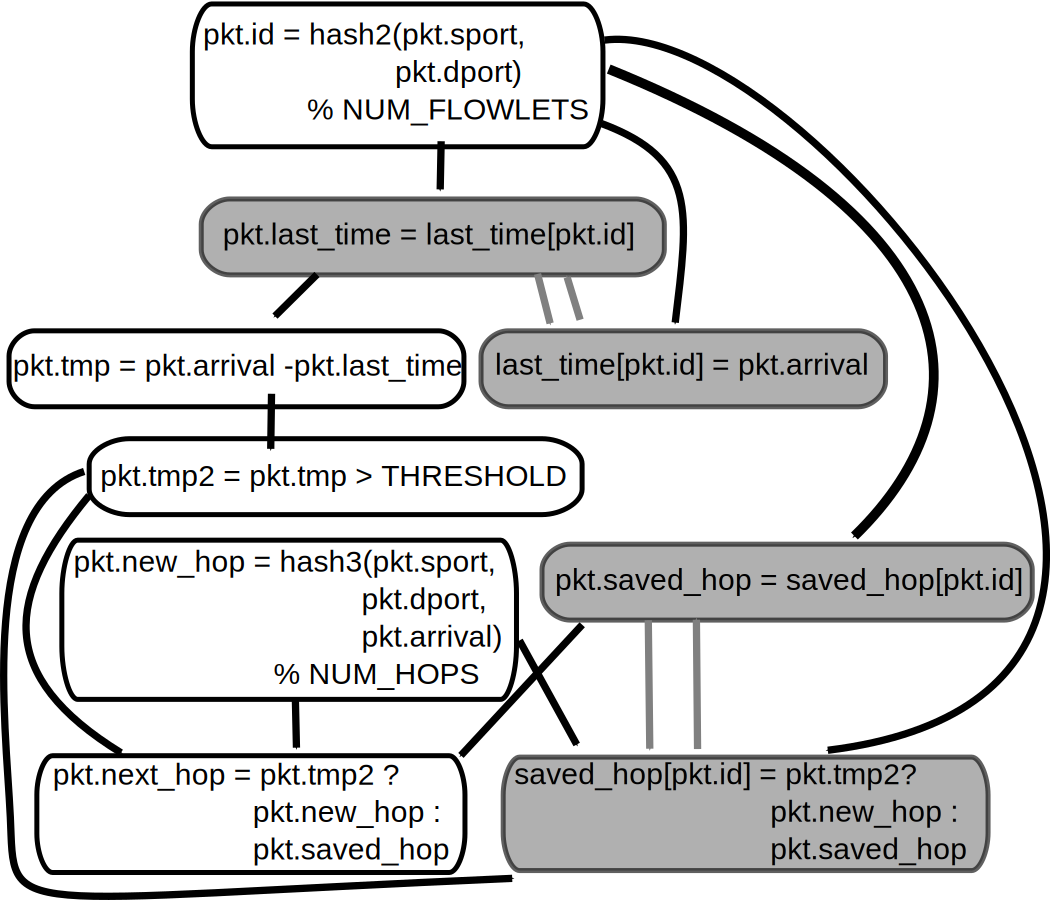
\includegraphics[width=\textwidth]{deps.pdf}
  \caption{Dependency graph of code shown in Figure~\ref{fig:three_address}}
  \label{fig:deps}
\end{figure*}

At this point, each strongly connected component can be turned into an atom for
\absmachine and the resulting pipeline implements the packet transaction.
Further, the atoms have a very stylized form. Stateless atoms contain exactly
one three-operand code instruction. Atoms that manipulate state contain at
least two statements: a read from a state variable and a write to a state
variable and optionally consist of one or more updates to the state variable.

\subsection{Constraints on atoms}
\label{ss:complexity}
So far, we haven't constrained the code in atom bodies in any way to reflect
hardware constraints. Expression flattening generates stateless atoms that each
have only one instruction. Further, because these instructions are in
three-operand code form, they map directly to the VLIW capabilities of
programmable switches.

Atoms that manipulate state can, in general, have multi-line atom bodies and it
is unclear whether these can be implemented at all. For instance, the update to
the state variable \texttt{saved\_hop} requires a read, followed by a
conditional update, followed by a write back. This section develops a general
technique to determine the implementability of stateful atoms, given
constraints on stateful atom bodies imposed by the hardware.

We first observe that constraints on stateful atoms can be written as program
sketches~\cite{bitstreaming, finite, sketch_manual}: a code fragment with fixed
and configurable parts. For instance, an atom with the constraint that it can
execute at most one programmable modify operation between a read and a write
operation to a stateful variable x can be represented as:
\begin{figure}
\begin{tiny}
\begin{lstlisting}
pkt.tmp = x;
pkt.tmp2 = pkt.tmp ?? (??);
x = pkt.tmp;
\end{lstlisting}
\end{tiny}
\caption{Sketch for single update operation to a state variable}
\label{fig:sketch_for_state}
\end{figure}
Here, the double question mark \texttt{??} stands for a
\textit{hole}~\cite{sketch_manual}. The hole is a placeholder for values from a
finite set that can be substituted in place of the hole. An automated program
synthesis~\cite{synthesis} tool called Sketch~\cite{sketch_manual} then
\textit{fills in} these holes to make the sketch equal to a specification.

As an example, if we want to implement the specification \texttt{x = x + 1;}
using the sketch in Figure~\ref{fig:sketch_for_state}, the Sketch tool would
fill the first hole with the value '+' from the finite set ('+', '-', '/', '*')
and the second hole with the value 1 from a finite set of integers specified as
input to the tool.

For the interested reader, a more detailed explanation of how Sketch works is
available in the appendix. For the purposes of the \pktlanguage compiler
though, we treat Sketch as a blackbox. We express the underlying constraints on
atoms as sketches, feed Sketch with an atom specification that needs to be
satisfied.  If there is a way to complete the sketch to satisfy the atom
specification, Sketch will find it, otherwise, it will determine that the
specification is unsatisfiable. For instance, the specification: \texttt{x = x
* x;} is unsatisfiable given the constraints in
Figure~\ref{fig:sketch_for_state}.

Using sketches to model constraints on atoms allows us to express constraints
very generically. At its core, a sketch is an incomplete imperative program,
and hence can express a variety of atom constaints. To show its generality, we
conside two such constraints in our evaluations: an in-order sequential CPU
that can execute exactly $N$ three-operand instructions and a combinatorial
circuit with a very specific form.

\begin{figure}
  \includegraphics[width=\columnwidth]{dag.pdf}
  \caption{DAG formed by condensing SCCs in Figure~\ref{fig:deps}}
  \label{fig:dag}
\end{figure}

%TODO: Maybe once we have enough examples of optimizations, we can roll those
%into SSA as saying how SSA makes it trivial to apply those optimizations.
% Again, this is compiler 101 for anyone who knows it.

\subsection{\tester: verifying compilations}

To conclude our description of the compiler, we describe our testing
infrastructure to verify that the compilation is correct i.e. the externally
visible behavior of the packet transaction (Figure~\ref{fig:flowlet}) is
indistinguishable from its pipelined implementation
(Figure~\ref{fig:pipeline}).

We verify correctness by feeding in the same set of test packets to both the
packet transaction and its implementation and comparing the outputs from both
programs on the set of externally visible fields. To create test packets, we
scan the packet transaction and generate the set of all packet fields read from
or written to by the transaction. We then initialize each of these fields by
sampling uniformly from the space of all 32-bit signed integers. In the future,
we plan to allow the user to specify more precise ranges for each packet field
that can be used for more directed testing.

To compare outputs from the packet transaction and its implementation, we track
renames that occur because of SSA. We compare each output field in the
transactional form with the last rename of the same output field in the
implementation. We then feed the same number of test packets to both the
specification and implementation and compare outputs at the end of the
pipeline. This allows to quickly ``spot check'' our compilations and was
instrumental in uncovering a few bugs in various compilation passes during
development.

\section{Evaluation}
\label{s:evaluation}
% Run some experiments with a stateless program.
% 1. We can compile more than one program (CRC16 checker).
% 2. We can compile more than one interesting program.
% 3. That the compilations actually works.
% 4. (Approximations can be omitted for now, punt to future work). 

We built a simple tick-based simulator to evaluate the correctness of
partitioning. Our simulator instantiates a configurable number of pipeline
stages and runs arbitrary code within each stage. To run the
original input transactional code, we create exactly one pipeline stage and run
the entire transactional code within it. \ac{I thought doing this would return 
incorrect results for flowlet.} To run our partitioned code, we create
as many pipeline stages as the number of partitions and run the code from each
partition within the corresponding pipeline stage. \ac{why do you need to do 
that if the compiler already generates partitioned P4 code as output?}

To simulate a variety of random packet inputs to our simulator, we use a
traffic source that samples from a Poisson distribution every clock tick.
While Poisson traffic is unrealistic, it provides sufficient randomness in
time-sensitive packet fields such as the enqueue and dequeue queue sizes,
queueing latencies, and interarrival times. In effect, this creates a set of
random test vectors that we can use to check if the partitioned code is correct
wrt the transactional specification.

\subsection{Correctness}
\label{ss:correctness}

The goal of this experiment is to check that our compiled \pktlanguage program
behaves the same as the original. 
We used Poisson traffic with an intensity of 0.3 and 0.7 packets per tick to
and generated 100000 packets to compare the transactional specification and
pipelined implementation of the flowlet switching. We also randomize the source
and destination ports used to determine the next hop in flowlet switching.

To check for correctness, we print out every packet at the end of all pipeline
stages (at the end of the single pipeline stage for the transactional
specification) and check if they are identical on every field. We used this
method to determine that the flowlet switching example is correctly
partitioned, with very high probability.
% TODO: Mention somewhere how this doesn't change anything. We could use a more
% involved computation like a Jenkins hash, it would just be more painful to show
% in the compiler.
% TODO: Be consistent between pipelined and partitioned.

\subsection{Approximating algorithms}
Present EWMA example. Show how
1. Without MAC instructions, you need to use recirculation, which leverages the approximate nature of EWMA.
2. With MAC instructions, you can do EWMA exactly.

\section{Related work}
\label{s:related}
NPUs: Tradeoffs are different here. Each stage can do very very little on a switch relative to an NPU. NPUs are Turing-complete; here, on a switch, programs either fit or don't. If they don't fit, you need to approximate.

P4 compiler (Lavanya's work): Complementary backend.

CMU work on pipelining datapaths: Verilog and circuits.

P4 itself: Too low level. NetASM: Once P4 needs an IR, NetASM might be a good choice.

Click: P4 paper wrote it off. We think its worth revisiting here.

Fastpass or Flexplane: Say that you love the abstraction they propose,
but would love to do it at higher line rates.

Click, Maple, Flexplane: Proposed transactions first. We are inspired by them.

\section{Future work}
\label{s:future}
1. Arrays and other aggregates.
2. Table layout: compiling to P4 and then go down. Make it the P4 compiler's problem.
TCP traffic and end-to-end evaluation of approximation quality like video quality in approximate computing.
So far our approach to evaluating approximations is empirical, not analytical. Analysis would be awesome.
3. Scheduling, by definition, requires looking at multiple packets together to
make a decision on what packet to schedule next, while data-plane algorithms
operate independenly on each packe


\bibliographystyle{abbrv} 
\begin{small}
\bibliography{hotnets15}
\end{small}
\label{last-page}

\end{document}

